\begin{figure*}[!htb]
    \centering
    \begin{tabular}[t]{c}%{|c|c|}
        %\hline
        \begin{subfigure}[t]{1.0\textwidth}
            \centering
            \caption{}
            
\includegraphics[width=\linewidth, trim=0cm 18cm -20cm 0.5cm]{fig/extract_viz_draw_position_untangle/chr6_pan_fa_a2fb268_4030258_6a1ecc2_smooth_mhc_H1000w120}
        \end{subfigure} \\
        \begin{tabular}{c}% if you add [t], then sub images are pushed down
            %\smallskip
            \begin{subfigure}[t]{0.5\textwidth}
                \centering
                \caption{}
                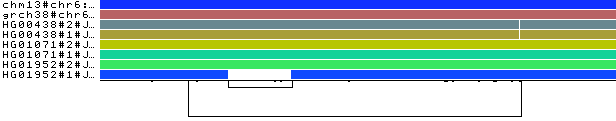
\includegraphics[width=\linewidth, trim=0 1.9cm 0cm 0cm]{fig/extract_viz_draw_position_untangle/chr6_pan_fa_a2fb268_4030258_6a1ecc2_smooth_C4_sorted}
            \end{subfigure} \\
            \begin{subfigure}[t]{0.5\textwidth}
                \centering
                \caption{}
                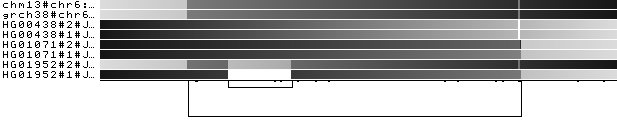
\includegraphics[width=\linewidth, trim=0 +1.9cm 0cm 0cm]{fig/extract_viz_draw_position_untangle/chr6_pan_fa_a2fb268_4030258_6a1ecc2_smooth_C4_sorted_du}
            \end{subfigure} \\
            \begin{subfigure}[t]{0.5\textwidth}
                \centering
                \caption{}
                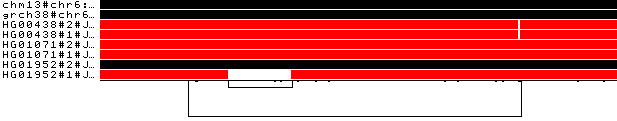
\includegraphics[width=\linewidth, trim=0 +1.9cm 0cm 0cm]{fig/extract_viz_draw_position_untangle/chr6_pan_fa_a2fb268_4030258_6a1ecc2_smooth_C4_sorted_z}
            \end{subfigure} \\
            \begin{subfigure}[t]{0.5\textwidth}
                \centering
                \caption{}
                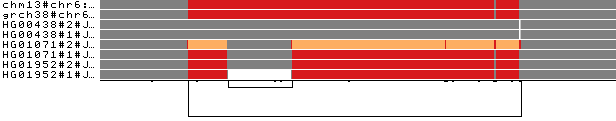
\includegraphics[width=\linewidth, trim=0 +1.9cm 0cm 0cm]{fig/extract_viz_draw_position_untangle/chr6_pan_fa_a2fb268_4030258_6a1ecc2_smooth_C4_sorted_m}
            \end{subfigure}
        \end{tabular}
        %&
        \begin{tabular}{c}% if you add [t], than sub images are pushed down
            %\smallskip
            \\\\
            \begin{subfigure}[t]{0.5\textwidth}
                \centering
                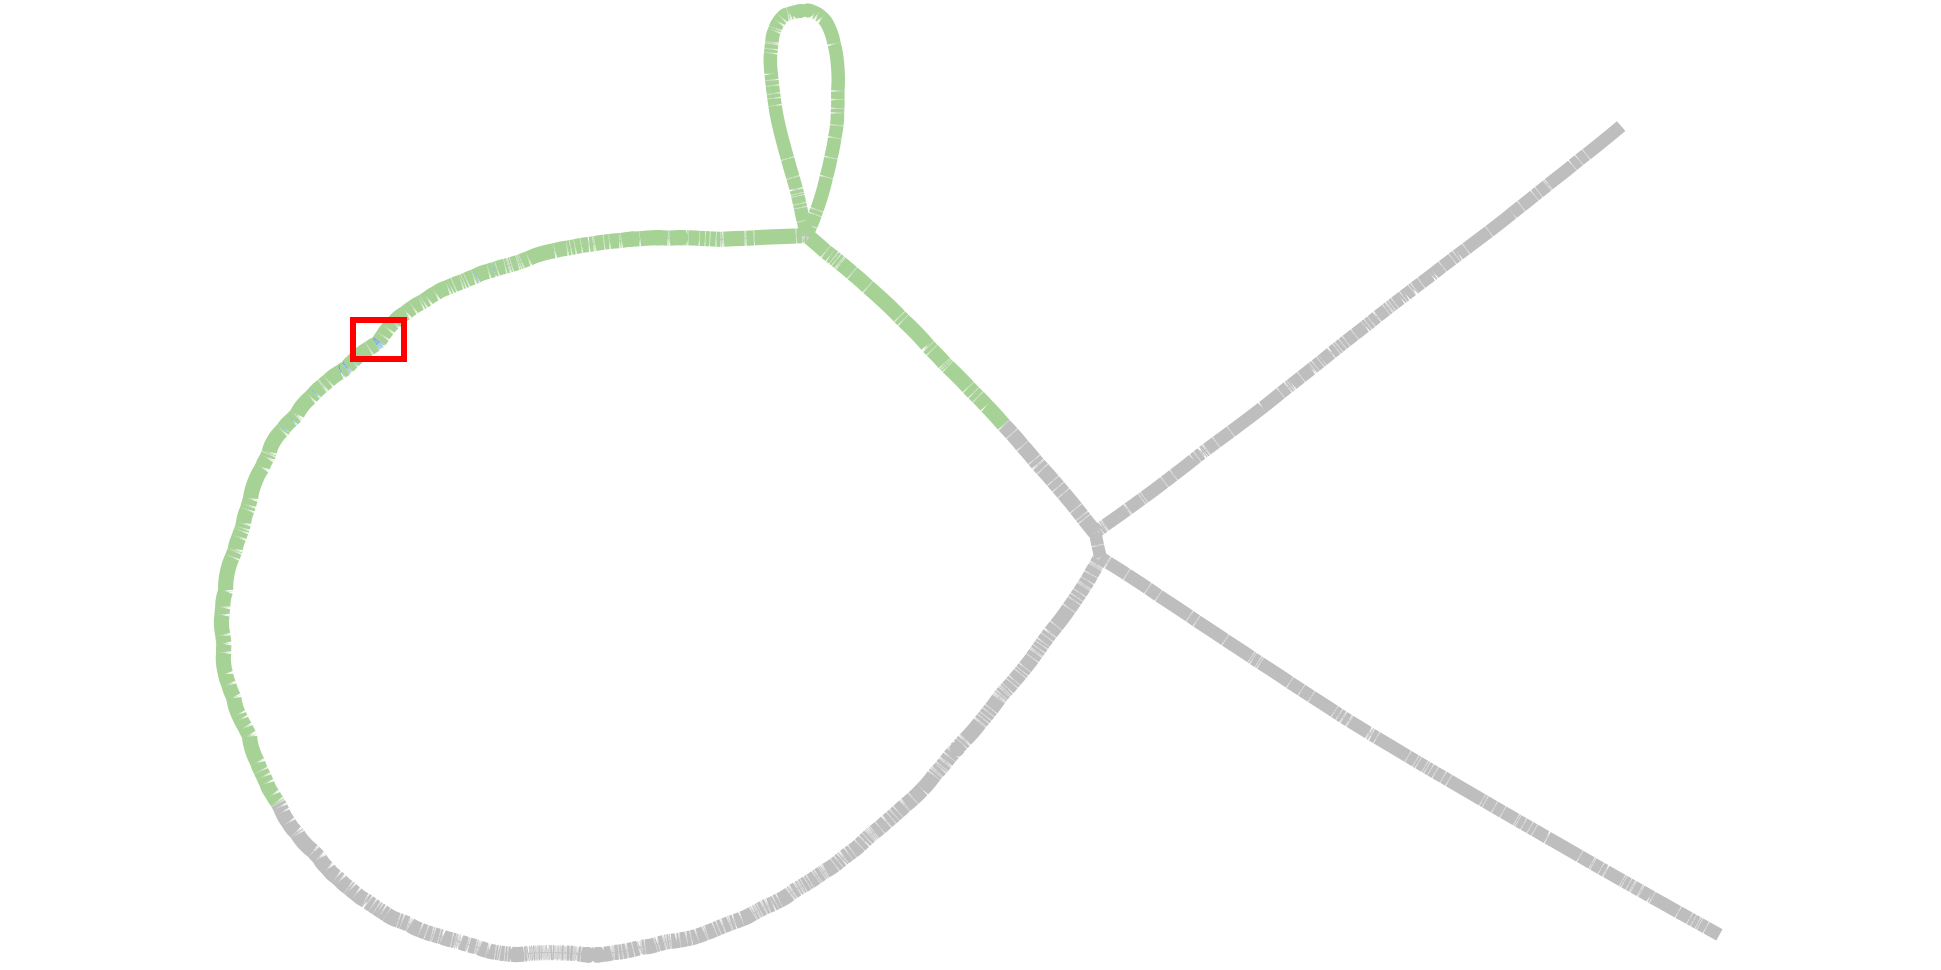
\includegraphics[width=0.65\linewidth, trim=0 +2cm 0 0.5cm]{fig/extract_viz_draw_position_untangle/chr6_pan_fa_a2fb268_4030258_d9f1245_smooth_gfa_C4_sorted_bandage}
                \caption{}
            \end{subfigure}
            \\\\
            \begin{subfigure}[t]{0.5\textwidth}
                \centering
                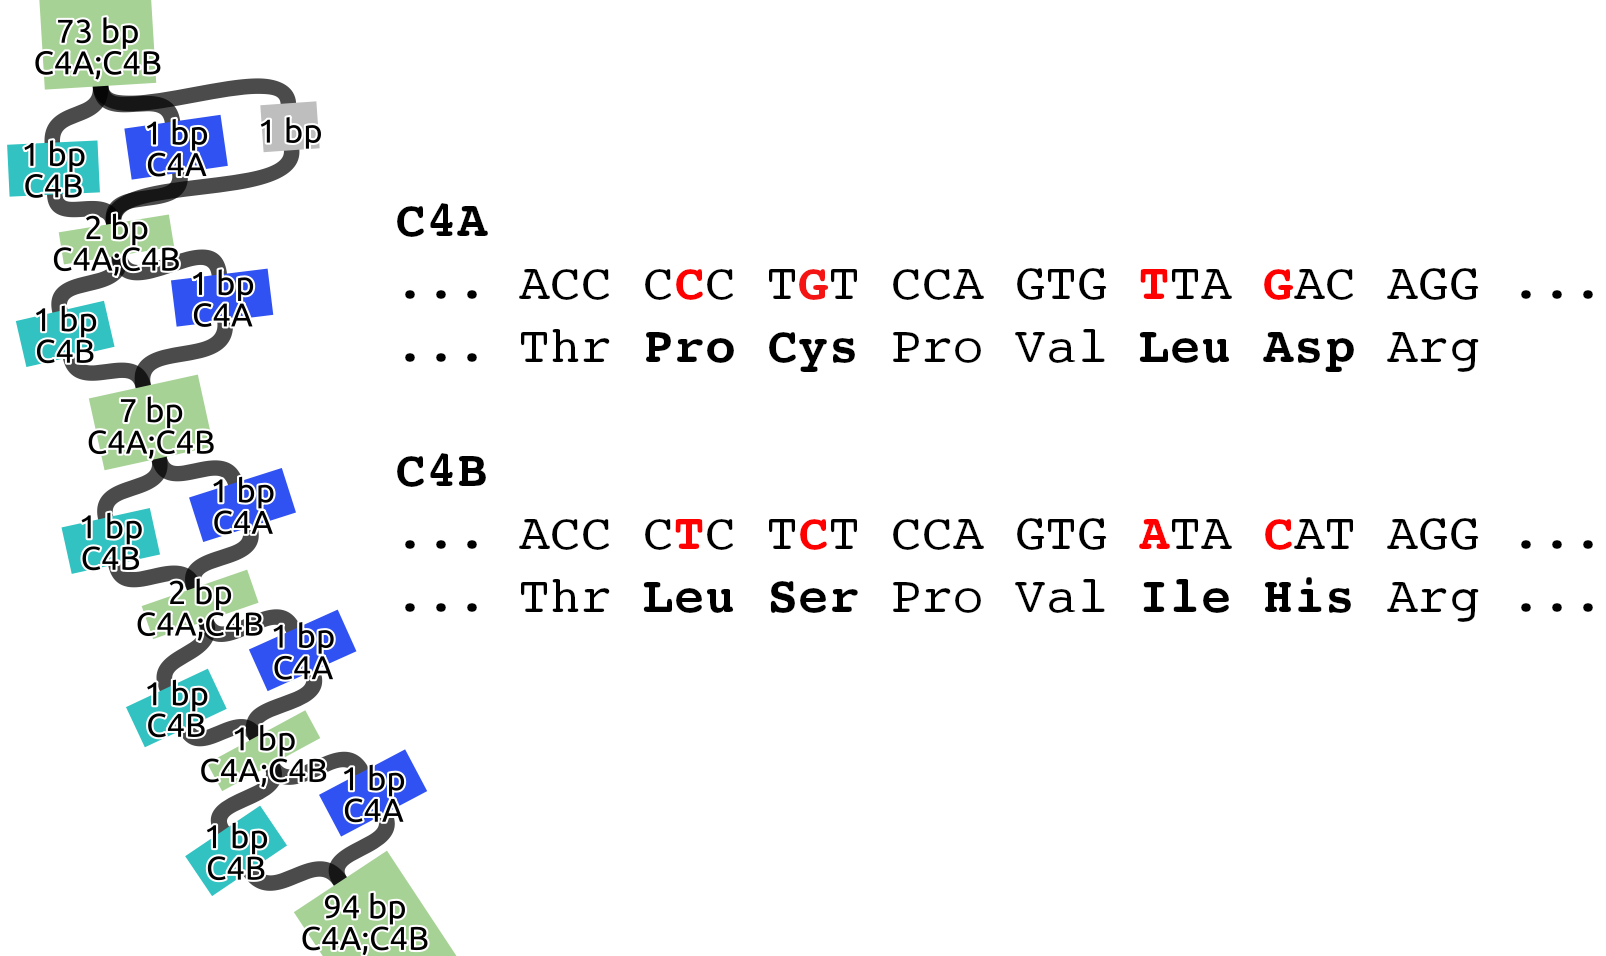
\includegraphics[width=0.65\linewidth, trim=0 +8cm 0 0.5cm]{fig/extract_viz_draw_position_untangle/chr6_pan_fa_a2fb268_4030258_d9f1245_smooth_gfa_C4_sorted_bandage_zoom_in}
                \caption{}
            \end{subfigure}
        \end{tabular}\\
        \begin{subfigure}[t]{1.0\textwidth}
            \centering
            \caption{}
            \begin{center}
                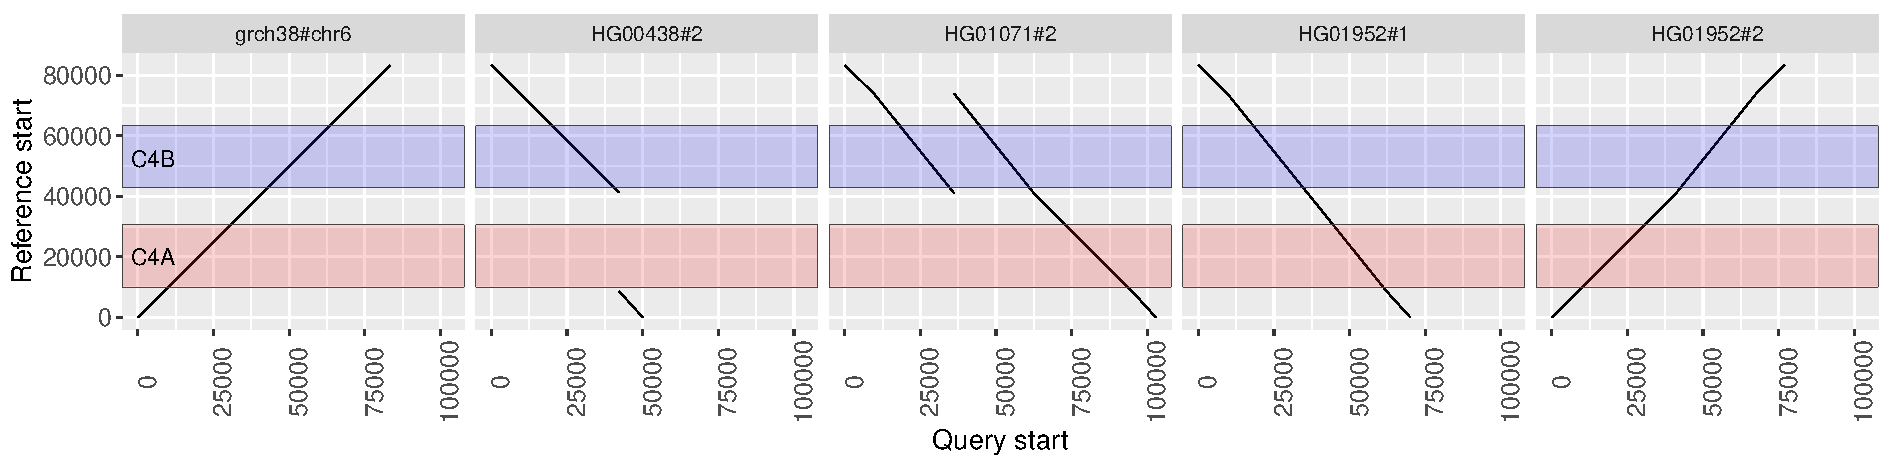
\includegraphics[width=\linewidth, trim=0cm 0.9cm -2.5cm 0.5cm]{fig/extract_viz_draw_position_untangle/chr6_pan_fa_a2fb268_4030258_6a1ecc2_smooth_C4_sorted_untangle_bed}
            \end{center}
        \end{subfigure} \\
        %\hline
    \end{tabular}
    \caption{
        Visualizing the MHC and C4 pangenome graphs. \textbf{(a)} \textit{odgi draw} layout of the MHC pangenome graph extracted from a whole human pangenome graph of 90 haplotypes. The red rectangle highlights the C4 region.
        \textbf{(b-e)} \textit{odgi viz} visualizations of the C4 pangenome graph, where 8 paths are displayed: 2 reference genomes (chm13 and grch38 on the top) and 6 haplotypes of 3 individuals.
        \textbf{(b)} \textit{odgi viz} default modality: the image shows a quite linear graph.
        The longer links at the bottom indicate the presence of a structural variant (long link) with another structural variant nested inside it (short link on the left).
        Indeed, human C4 exists as 2 functionally distinct genes, \textit{C4A} and \textit{C4B}, which both vary in structure and copy number~\citep{Sekar_2016}. The longer link indicates that the copy number status varies across the haplotypes represented in the pangenome.
        Moreover, \textit{C4A} and \textit{C4B} genes segregate in both long and short genomic forms, distinguished by the presence or absence of a human endogenous retroviral (HERV) sequence, as also highlighted by the short nested link on the left.
        \textbf{(c)} Color by path position. %: the color gradients are smooth, highlighting that its node are well sorted in 1 dimension.
        The top two reference genomes and 2 haplotypes (HG01952\#2) go from left to right, while 5 haplotypes go in the opposite direction, as indicated by the black color on their left.
        \textbf{(d)} \textit{odgi viz} color by strandness: the red paths indicate the haplotypes that were assembled in reverse with respect to the 2 reference genomes.
        \textbf{(e)} \textit{odgi viz} color by path depth: using the Spectra color palette with 4 levels of path depths, white indicates no depth, while grey, red, and yellow indicate depth 1, 2, and greater than or equal to 3, respectively.
        Coloring by path depth, we can see that the two references present two different allele copies of the C4 genes, both of them including the HERV sequence.
        The entirely grey paths have one copy of these genes.
        HG01071\#2 presents 3 copies of the \textit{locus} (orange), of which one contains the HERV sequence (gray in the middle of the orange).
        In HG01952\#1, the HERV sequence is absent.
        \textbf{(f)} \textit{Bandage}~\citep{Wick_2015} layout of the C4 pangenome graph, annotated by using \textit{odgi position}. Green nodes indicate the C4 genes. The red rectangle highlights the regions where \textit{C4A} and \textit{C4B} genes differ.
        \textbf{(g)} Annotated \textit{bandage} layout of the C4 region where \textit{C4A} and \textit{C4B} genes differ due to single nucleotide variants leading to changes in the encoded protein sequences. Node labels were annoted by using \textit{odgi position}.
        \textbf{(h)} Visualization of \textit{odgi untangle} output in the C4 pangenome graph: the plots show the copy number status of the sequences in the C4 region with respect to the grch38 reference sequence, making clear, for example, that in HG00438\#2, the \textit{C4A} gene is missing. \vspace{-1em}
    }
    \label{fig:odgi_viz}
\end{figure*}


%\begin{figure*}[h!]
%    \begin{subfigure}[t]{.50\linewidth}
%        \caption{}
%        \centering
%        % include first image
%        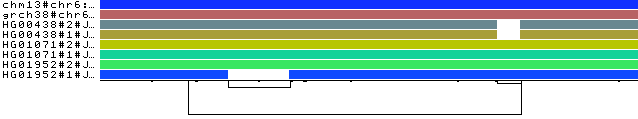
\includegraphics[width=\linewidth, trim=0 +1.5cm -0.5cm 0.5cm]{fig/extract_viz_draw_position_untangle/chr6_pan_fa_a2fb268_4030258_d9f1245_smooth_gfa_C4_sorted}
%        \label{fig:odgi_viz_default}
%    \end{subfigure}
%
%    \begin{subfigure}[t]{.50\linewidth}
%        \caption{}
%        \centering
%        % include second image
%        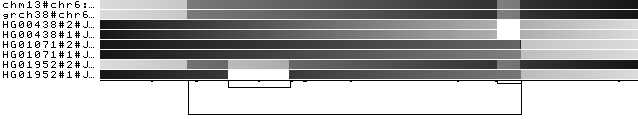
\includegraphics[width=\linewidth, trim=0 +1.5cm -0.5cm 0.5cm]{fig/extract_viz_draw_position_untangle/chr6_pan_fa_a2fb268_4030258_d9f1245_smooth_gfa_C4_sorted_du}
%        \label{fig:odgi_viz_color_by_path_pos}
%    \end{subfigure}
%
%    \begin{subfigure}[t]{.50\linewidth}
%        \caption{}
%        \centering
%        % include second image
%        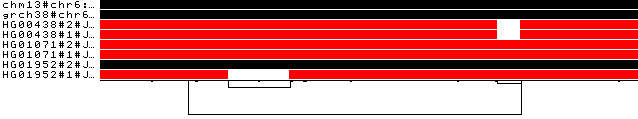
\includegraphics[width=\linewidth, trim=0 +1.5cm -0.5cm 0.5cm]{fig/extract_viz_draw_position_untangle/chr6_pan_fa_a2fb268_4030258_d9f1245_smooth_gfa_C4_sorted_z}
%        \label{fig:odgi_viz_color_by_inversion_rate}
%    \end{subfigure}
%
%    \begin{subfigure}[t]{.50\linewidth}
%        \caption{}
%        \centering
%        % include fourth image
%        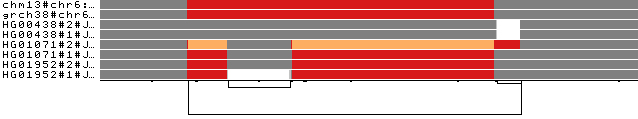
\includegraphics[width=\linewidth, trim=0 +1.5cm -0.5cm 0.5cm]{fig/extract_viz_draw_position_untangle/chr6_pan_fa_a2fb268_4030258_d9f1245_smooth_gfa_C4_sorted_m}
%        \label{fig:odgi_viz_color_by_path_depth}
%    \end{subfigure}
%    \begin{subfigure}[t]{.50\linewidth}
%        \caption{}
%        \centering
%        % include first image
%        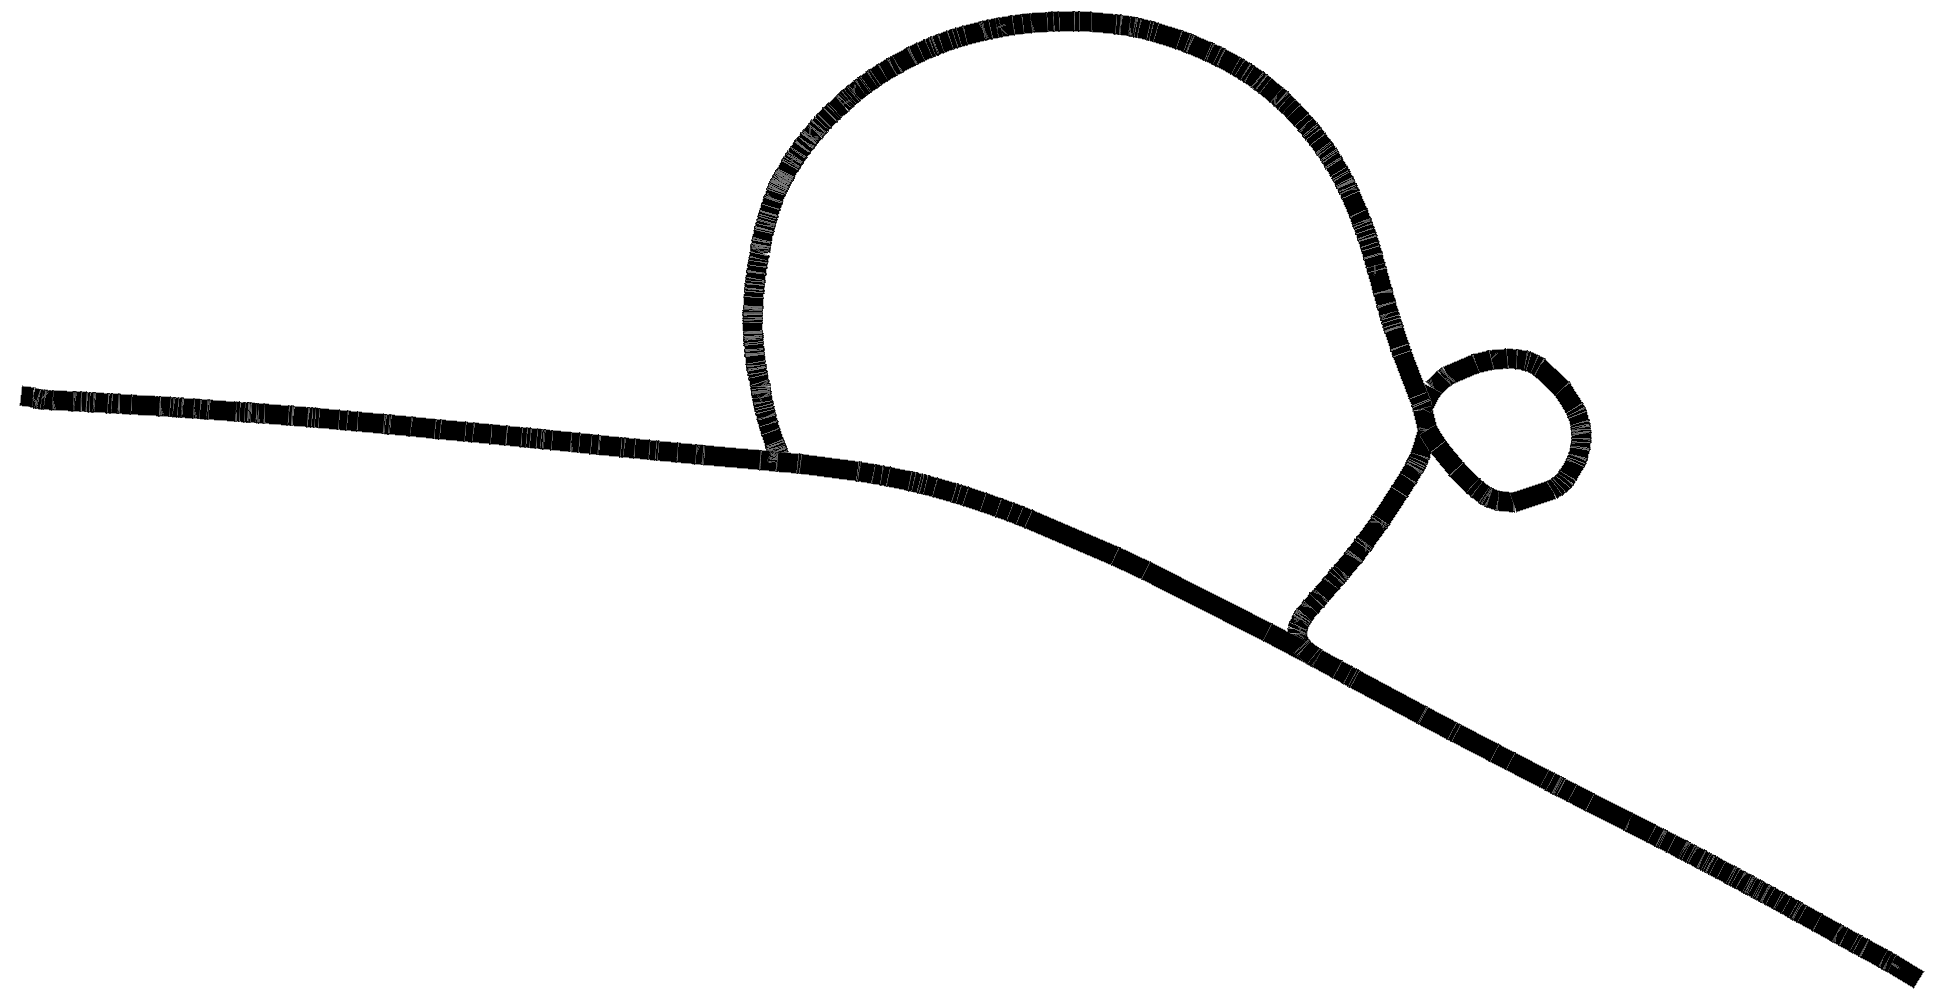
\includegraphics[width=0.5\linewidth, trim=0 +2cm 0 0.5cm]{fig/extract_viz_draw_position_untangle/chr6_pan_fa_a2fb268_4030258_d9f1245_smooth_gfa_C4_sorted_layout}
%        \label{fig:odgi_viz_default2}
%    \end{subfigure}
%    \begin{subfigure}[t]{.50\linewidth}
%        \caption{}
%        \centering
%        % include second image
%        %todo BANDAGE
%        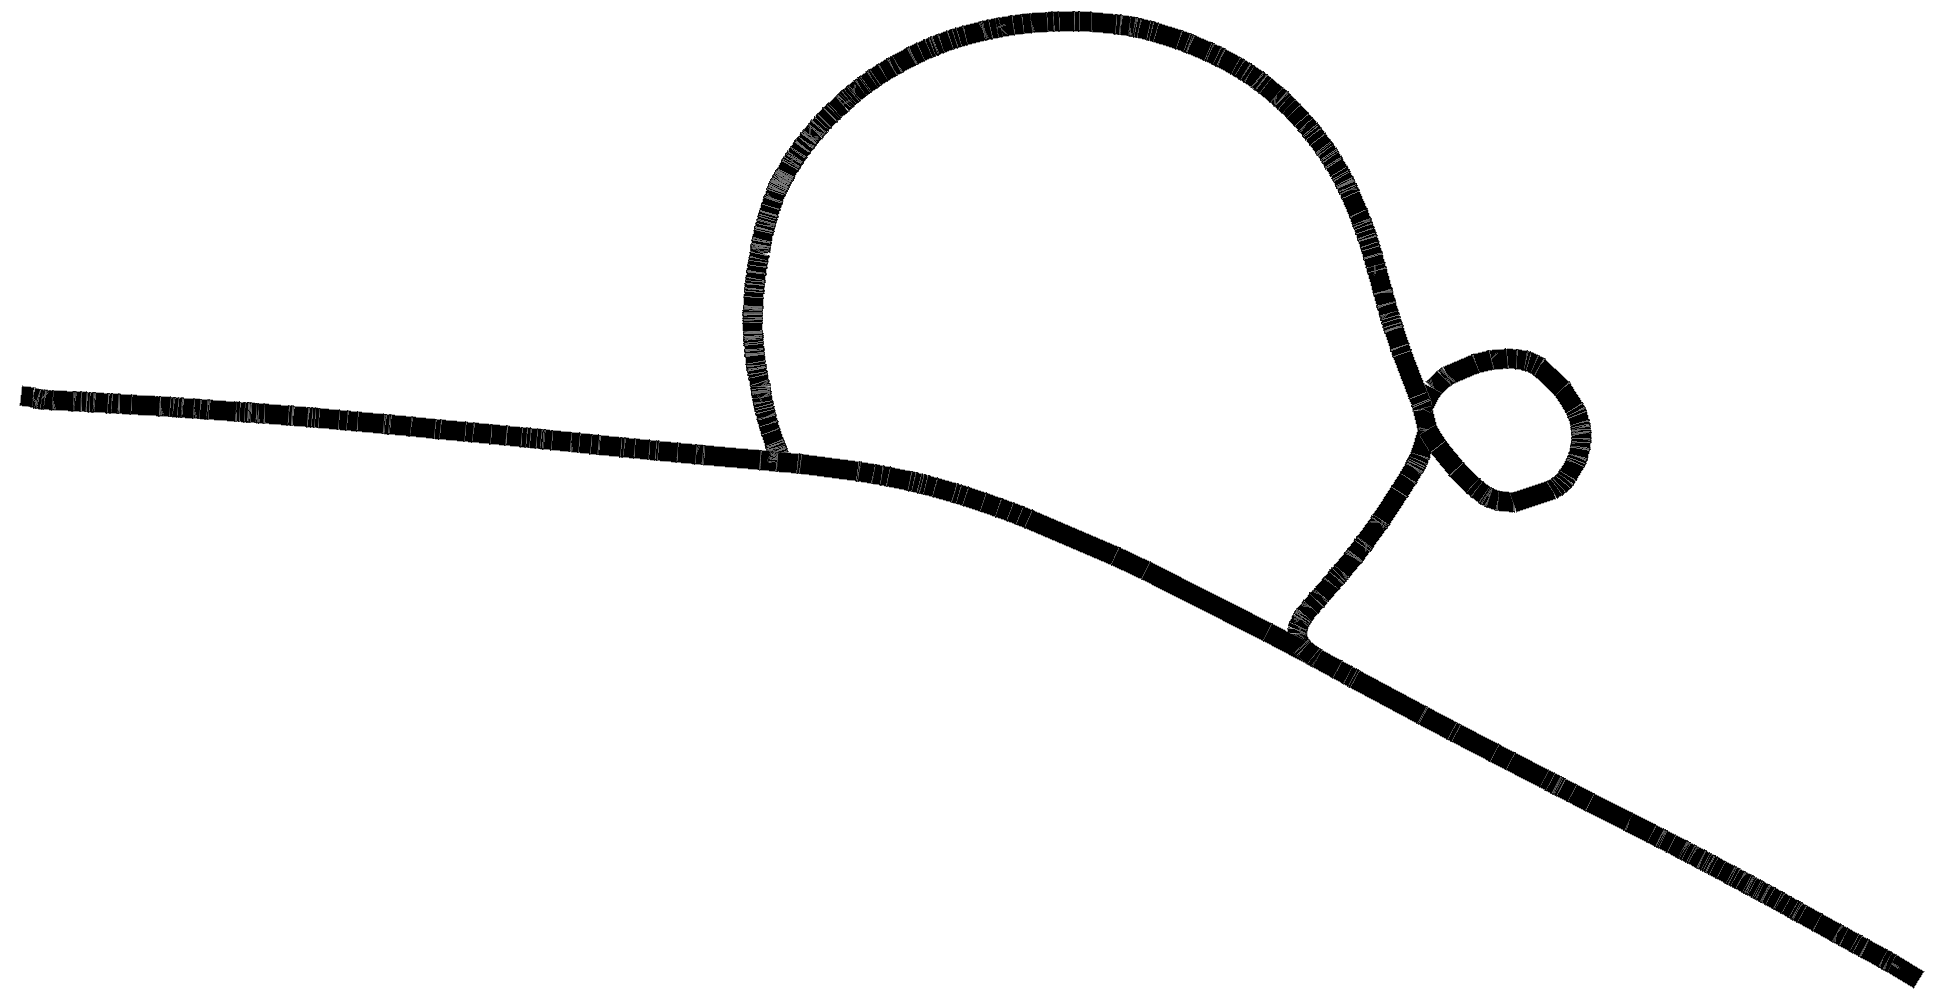
\includegraphics[width=0.5\linewidth, trim=0 +1.5cm -0.5cm 0.5cm]{fig/extract_viz_draw_position_untangle/chr6_pan_fa_a2fb268_4030258_d9f1245_smooth_gfa_C4_sorted_layout}
%        \label{fig:odgi_viz_color_by_inversion_rate2}
%    \end{subfigure}
%
%    \caption{
%        Visualizing the complement component 4 (C4) pangenome graph extracted from a whole human pangenome graph of 90 haplotypes.
%        In all visualizations, 8 paths are displayed: 2 reference genomes (chm13 and grch38 on the top) and 6 haplotypes of 3 individuals.
%        \textbf{(a)} default modality: the image shows a quite linear graph.
%        The longer links at the bottom indicate the presence of a structural variant (long link) with another structural variant nested inside it (short link on the left).
%        Indeed, human C4 exists as 2 functionally distinct genes, C4A and C4B, which both vary in structure and copy number \citep{Sekar_2016}. The longer link indicates that the copy number status varies across the haplotypes represented in the pangenome.
%        Moreover, C4A and C4B genes segregate in both long and short genomic forms, distinguished by the presence or absence of a human endogenous retroviral (HERV) sequence, as also highlighted by the short nested link on the left.
%        \textbf{(b)} color by path position: the color gradients are smooths, highlighting that its node are well sorted in 1 dimension.
%        The top two reference genomes and 2 haplotypes (with name starting with HG01952\#2) go from left to right, while 5 haplotypes go in the opposite direction, as indicated by the black color on their left.
%        \textbf{(c)} color by strandness: the red paths indicate the haplotypes that were assembled in reverse with respect to the 2 reference genomes.
%        \textbf{(d)} color by path depth: using the Spectra color palette with 4 level of path depths, white indicates no depth, while grey, red, and yellow indicate depth 1, 2, and greater than or equal to 3, respectively.
%        Coloring by path depth, we can see that the two references present two different allele copies of the C4 genes, both of them including the HERV sequence.
%        The entirely grey paths have one copy of these genes.
%        The path with name starting with HG01071\#2 presents 3 copies of the genes (indicated by the orange color), of which only 1 with the HERV sequence (gray color in the middle of the orange region).
%        In the haplotype with the name starting with HG01952\#1, the HERV sequence is absent.
%    }
%    \label{fig:odgi_viz}
%\end{figure*}